\documentclass[12pt]{article}\usepackage[margin=1in]{geometry}\usepackage{amsmath,amssymb,amsthm,graphicx,natbib,microtype}\newtheorem{theorem}{Theorem}\newtheorem{corollary}[theorem]{Corollary}
\title{Spectral Normalization and Capacity Transport\\\large Sharp Gram-Comparison Exponents and the Cost of Separate Factors}\author{Prime Dynamics Theory Program}\date{July 2026}
\begin{document}\maketitle
\begin{abstract}
Suppose $mK^*K\preceq K'^*K'\preceq MK^*K$ and put $r=m/M$.  We prove sharp cross-level factors: $q_4'\geq r^{1/2}q_4$, normalized four-volume $\nu_4'\geq r^{3/2}\nu_4$, and three-mode capacity $r\Lambda_{23}\leq\Lambda_{23}'\leq r^{-1}\Lambda_{23}$.  Consequently, transporting volume and capacity as independent black boxes yields only $r^{5/2}q_4$, an extra loss $r^2$ relative to direct fourth-mode transport.  All powers are sharp in separate diagonal families.  A 4,096-instance audit has zero failures.  This theorem fixes the normalization ledger but assumes, rather than proves, physical all-level Gram comparability.
\end{abstract}
\section{Normalized quantities}
Let $s_1\geq s_2\geq\cdots$ be singular values and set
\[
q_4=\frac{s_4}{s_1},\quad \Lambda_{23}=\frac{s_2s_3}{s_1^2},\quad \nu_4=\frac{s_2s_3s_4}{s_1^3}=\Lambda_{23}q_4.
\]
The last identity is the RH-110 factor ledger.  Two-sided Gram comparison
implies $\sqrt m,s_j(K)\leq s_j(K')\leq\sqrt M,s_j(K)$ by ordered
eigenvalue monotonicity \citep{HornJohnson1991,Bhatia2007}.

\begin{theorem}[Sharp normalized transport]\label{thm:transport}
Under $mK^*K\preceq K'^*K'\preceq MK^*K$, with $r=m/M$,
\[
r^{1/2}q_4\leq q_4'\leq r^{-1/2}q_4,
\]
\[
r\Lambda_{23}\leq\Lambda_{23}'\leq r^{-1}\Lambda_{23},\qquad
r^{3/2}\nu_4\leq\nu_4'\leq r^{-3/2}\nu_4.
\]
Every displayed one-sided exponent is sharp.
\end{theorem}
\begin{proof}
Insert the singular-value bounds into each quotient after cancelling the
common leading factor.  Sharpness follows by diagonal scalings: use
$\sqrt M$ on $s_1$ and $\sqrt m$ on $s_4$ for $q_4$; use $\sqrt M$ on
$s_1$ and $\sqrt m$ on $s_2,s_3,s_4$ for $\nu_4$; reverse the first three
choices for the capacity upper.  The opposite bounds are analogous.
\end{proof}

\begin{corollary}[Separate-factor penalty]
If one forgets the common operator and combines only
$\nu_4'\geq r^{3/2}\nu_4$ with
$\Lambda_{23}'\leq r^{-1}\Lambda_{23}$, then
\[
q_4'=\frac{\nu_4'}{\Lambda_{23}'}\geq r^{5/2}q_4.
\]
This is weaker than the direct $r^{1/2}$ bound by exactly $r^2$.
\end{corollary}
The corollary is not a contradiction: separate sharp bounds need not be
simultaneously attained.  It quantifies the price of discarding correlation.

\section{Audit and consequence}
We sample 4,096 source spectra, condition ratios spanning six decades, and
independent singular scalings inside $[\sqrt m,\sqrt M]$.  There are zero
$q_4$, capacity, or volume failures.  Three diagonal records attain the
corresponding sharp factors.
\begin{figure}[h]\centering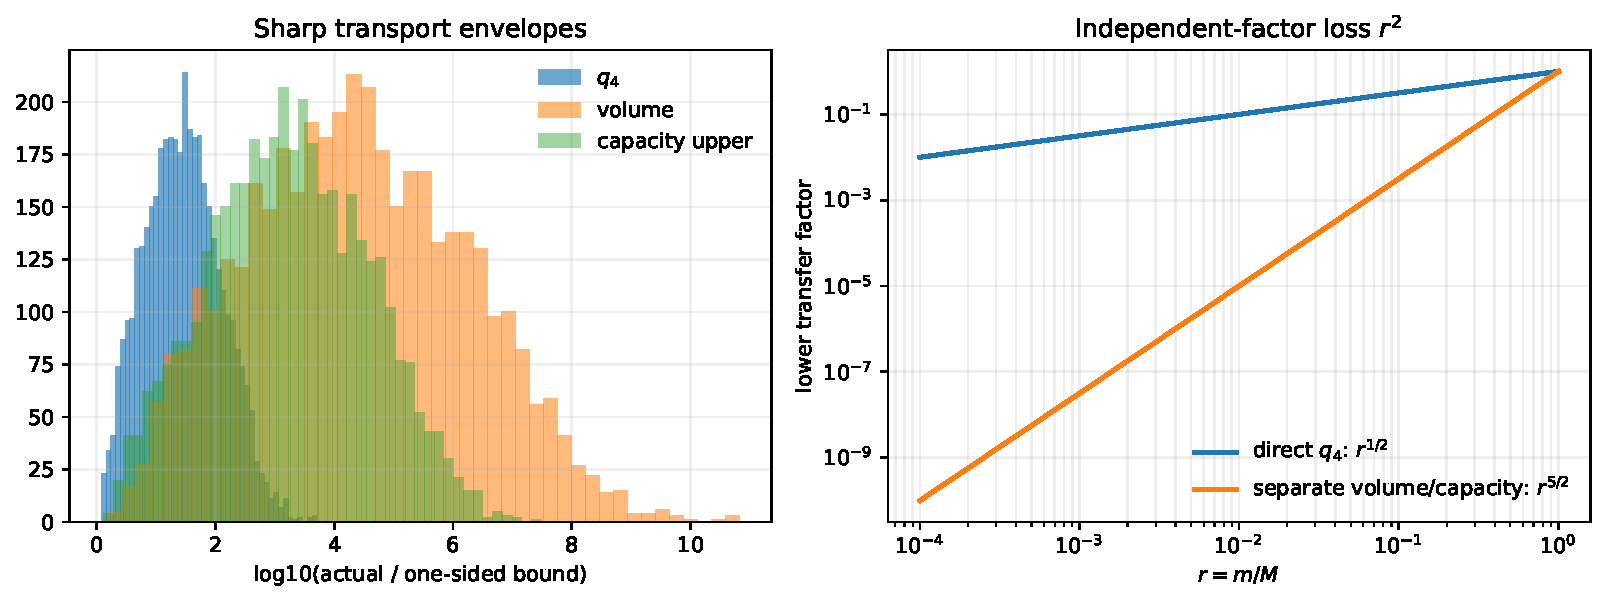
\includegraphics[width=\textwidth]{figures/spectral_normalization_capacity_transport.pdf}\caption{Transport-envelope efficiency and the $r^2$ loss caused by separate factorization.}\end{figure}
RH-124 shows that a combined directional theorem should preserve common
cross-level information whenever possible.  It does not supply physical
$m,M$ constants.  No uniform Stage A, Hilbert--Polya operator, zeta-zero
identification, or Riemann Hypothesis conclusion is claimed.
\bibliographystyle{plainnat}\bibliography{references}\end{document}
